\chapter{The parallel model}
\label{ch:parallel}

\section{Decomposition}

The global box $[\vect{x}_{\min},\vect{x}_{\max})$ is divided into
$\texttt{cuts[0]}\times\texttt{cuts[1]}\times\texttt{cuts[2]}$ sub-boxes, one per rank. With
\fn{MFTLEnsembleCreate} the division is uniform and sub-box $(i,j,k)$ belongs to the rank that
the MPI Cartesian communicator assigns to it; with \fn{MFTLEnsembleCreateRectilinear} the slab
coordinates along every axis (\texttt{axis\_cuts}) and the map from sub-box to rank
(\texttt{rank\_map}) are given explicitly. The domain stores the box, its size
$\vect{L}=\vect{x}_{\max}-\vect{x}_{\min}$ (\texttt{domain\_size}), half of it
(\texttt{domain\_half\_size}, the minimum-image threshold), the periodicity per axis, and the
de-duplicated list of the ranks owning the up to 26 neighbouring sub-boxes
(\texttt{neighbors}). On a periodic axis with one or two slabs a rank may be its own
neighbour, or the same rank may be the neighbour on both sides; the library handles both.

The owner of a point is the rank of the sub-box that contains it:
\begin{lstlisting}[numbers=none]
static inline int MFTLGetOwnerProc(const MFTL_Domain *domain, const double pos[3]);
\end{lstlisting}
Points on an internal slab face belong to the upper slab; points outside the box are clamped
to the first or last slab. During load-balanced remeshing a temporary x-only ownership
(\texttt{lb\_nprocs}, \texttt{lb\_xcuts}) replaces the Cartesian map (\S\ref{sec:parallel-remesh}).

\section{Ownership}

Every entity has exactly one owner, the only rank whose copy is authoritative:
\begin{itemize}
  \item a \emph{vertex} is owned by the rank that owns its position \texttt{pos};
  \item a \emph{triangle} is owned by the rank that owns its \emph{cached} centre
    \texttt{center} (the centroid of its corners, wrapped into the box);
  \item a \emph{half-edge} belongs to its triangle.
\end{itemize}
Copies on other ranks are \emph{ghosts}: \texttt{is\_ghost} is set and \texttt{owner\_proc} names
the owner. Ghosts are read-only: they exist so that the owner of a vertex can see the whole fan
around it and so that the owner of a triangle can see its neighbours. A value written into a
ghost is overwritten at the next refresh. Integrals and statistics count owned entities only.

Because the triangle owner is taken from the cached centre, \fn{MFTLComputeTriangleProperties}
must be called after positions have changed and before a redistribution. The transforms of
Chapter~\ref{ch:geometry} and the remesher do this themselves; an application that moves
vertices itself calls it explicitly (see the listings of Chapter~\ref{ch:examples}).

\section{Redistribution}

\begin{lstlisting}[numbers=none]
int MFTLRedistribute(MFTL_Ensemble *ens);             /* all objects of the ensemble */
int MFTLRedistributeObject(MFTL_Object *object);      /* one object */
int MFTLRedistributeListOfObjects(MFTL_Ensemble *ensemble);
\end{lstlisting}
A redistribution (collective) recomputes the owner of every entity from its current position
(vertices) or cached centre (triangles) and moves it there. Each triangle is sent to its owner,
to the owners of its three vertices and to the owners of its edge-neighbour triangles, so every
rank receives one layer of ghosts around its owned part (Figure~\ref{fig:distribution}). Global
ids, image counters, flags, the cached triangle geometry, the surface scalar and the opaque
payload travel with the entities; local indices are rebuilt.

On return the ensemble is at a \emph{quiescent point}:
\begin{itemize}
  \item every entity is owned exactly once, and the owned entities are stored first;
  \item every edge of an owned triangle is LOCAL or BOUNDARY (ghost completion G1) and the
    fan of every owned vertex is stored completely (G2), \S\ref{sec:completion};
  \item the twin states have been validated (\S\ref{sec:validation}).
\end{itemize}
On a single rank a redistribution does nothing and returns \texttt{MFTL\_SUCCESS}. It returns
\texttt{MFTL\_ERROR} on a payload-size mismatch between ranks or when ghost completion or
validation fails. \fn{MFTLRedistribute} calls \fn{MFTLRedistributeObject} for an ensemble with
one object and \fn{MFTLRedistributeListOfObjects} otherwise; the latter moves all objects in
one communication round.

\begin{figure}[ht]
\centering
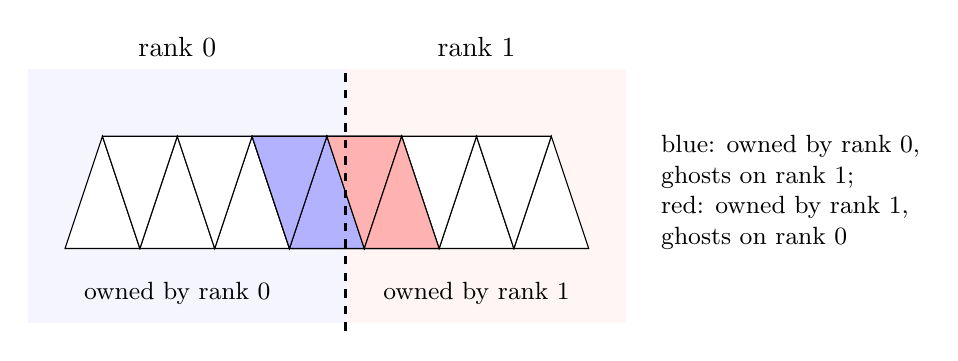
\begin{tikzpicture}[scale=0.95]
  \fill[blue!4] (0,0) rectangle (4.25,3.4); \fill[red!4] (4.25,0) rectangle (8,3.4);
  \node at (2,3.7) {rank 0}; \node at (6,3.7) {rank 1};
  % strip: bottom vertices (x,1), top vertices (x+0.5,2.5); up-triangles i, down-triangles i
  \foreach \x in {0.5,1.5,...,6.5} { \filldraw[fill=white,draw=black] (\x,1) -- (\x+1,1) -- (\x+0.5,2.5) -- cycle; }
  \foreach \x in {0.5,1.5,...,5.5} { \filldraw[fill=white,draw=black] (\x+0.5,2.5) -- (\x+1.5,2.5) -- (\x+1,1) -- cycle; }
  % triangles next to the slab face: owned left of it (blue), right of it (red); each stored on both ranks
  \filldraw[fill=blue!30,draw=black] (3.5,1) -- (4.5,1) -- (4,2.5) -- cycle;
  \filldraw[fill=blue!30,draw=black] (3,2.5) -- (4,2.5) -- (3.5,1) -- cycle;
  \filldraw[fill=red!30,draw=black] (4,2.5) -- (5,2.5) -- (4.5,1) -- cycle;
  \filldraw[fill=red!30,draw=black] (4.5,1) -- (5.5,1) -- (5,2.5) -- cycle;
  \draw[very thick,dashed] (4.25,-0.1) -- (4.25,3.4);
  \node[font=\small] at (2,0.4) {owned by rank 0};
  \node[font=\small] at (6,0.4) {owned by rank 1};
  \node[align=left,font=\small] at (10.2,1.75) {blue: owned by rank 0,\\ ghosts on rank 1;\\ red: owned by rank 1,\\ ghosts on rank 0};
\end{tikzpicture}
\caption{Distribution with one ghost layer. A triangle is owned by the rank containing its
centre; the triangles next to the slab face are also stored on the other rank as ghosts, so
that each rank sees the complete fan of every vertex it owns.}
\label{fig:distribution}
\end{figure}

\section{Refreshing ghosts}

Moving owned vertices leaves the ghost copies on other ranks stale. Two collective refreshes
update ghosts without changing which entities are stored:
\begin{itemize}
  \item \fn{MFTLUpdateGhostPositions}\texttt{(ens, lookup)} copies, for every ghost vertex, the
    owner's position, image counters, normal, curvatures, area and roughness;
  \item \fn{MFTLScatterTriangleData}\texttt{(ens, lookup)} copies the owner's opaque payload into
    every ghost triangle (Chapter~\ref{ch:data}).
\end{itemize}
Both exchange data with the graph neighbours only. A ghost whose owner is not a graph neighbour
any more (because a vertex moved further than a slab, or during parallel remeshing) stays stale
until the next redistribution; the call prints how many such ghosts it met. The argument
\texttt{lookup} is an optional hash map from object id to object index (\texttt{MFTL\_NULL}:
linear search).

Cached triangle properties of ghost triangles are \emph{not} refreshed by either call: they are
set by the owner and travel with the triangle at the next redistribution. The recommended
sequence after moving vertices is therefore
\begin{lstlisting}[numbers=none]
/* move owned vertices ... */
MFTLUpdateGhostPositions(ens, MFTL_NULL);   /* ghost vertices follow their owners      */
MFTLComputeTriangleProperties(obj);         /* cached area/normal/centre of owned tris */
MFTLRedistribute(ens);                      /* new owners, fresh ghost layer           */
\end{lstlisting}

\section{Additional ghost layers and spatial ghosts}

\fn{MFTLExtendGhostLayer}\texttt{(ens, steps)} imports further rings of ghost triangles
(\texttt{steps} layers) around the owned part, for kernels with a wider stencil than the one-ring.
Two functions import triangles by proximity rather than by topology:
\fn{MFTL\_CreateSpatialGhosts}\texttt{(objA, objB)} ships the owned triangles of one object whose
box meets the other object's box on a neighbour rank (periodic-aware box tests; used by the
intersection driver, \S\ref{sec:intersection}), and
\fn{MFTLEnsembleCreateSpatialGhosts}\texttt{(ens, tol)} ships owned triangles whose box, inflated by
\texttt{tol}, overlaps a neighbour rank's box (a plain box test on the stored positions, not
periodic-aware). \fn{MFTLObjectSendLocalTrianglesToAll}\texttt{(obj, distance)} makes every owned
triangle a ghost on \emph{every} rank whose box lies within \texttt{distance} of it (a global
exchange, not limited to the graph neighbours).

\section{Collective discipline}

Every collective function must be entered by all ranks of the ensemble in the same order.
Functions whose result depends on a point or a parameter (point queries, phase-set queries,
remesh parameters) require the same value on every rank. Inside the library, decisions that end loops or select algorithms are reduced over all ranks
before they are taken, so that no rank leaves a sequence of collectives early (see, for example,
the volume recovery of \S\ref{sec:volume-recovery}). One known defect violates this rule
(\S\ref{sec:known-defects}).
